\documentclass[10pt]{article}
\usepackage{amsmath}
\usepackage{amsfonts}
\usepackage{graphicx}

\setlength{\oddsidemargin}{0pt}
\setlength{\evensidemargin}{0pt}
\setlength{\textwidth}{6.5in}
\setlength{\topmargin}{0in}
\setlength{\textheight}{8.5in}

\setlength{\parskip}{1pc}
\setlength{\parindent}{0pt}

\newcommand{\ans}[1]{\textbf{#1}}

\begin{document}

\section*{Short Answers}

\subsection*{RTT}

\begin{enumerate}
\item Questions on experiment a:

\begin{itemize}
\item What percentage of the websites do not respond to pings at all? What percentage have at least one failed ping?

19\% of the websites do not respond to pings at all. 25\% of the websites have at least one failed ping.

\item Using the plot functions and \texttt{rtt\_a\_agg.json}, please plot a CDF of the median RTT of the websites that respond to ping.

\begin{center}
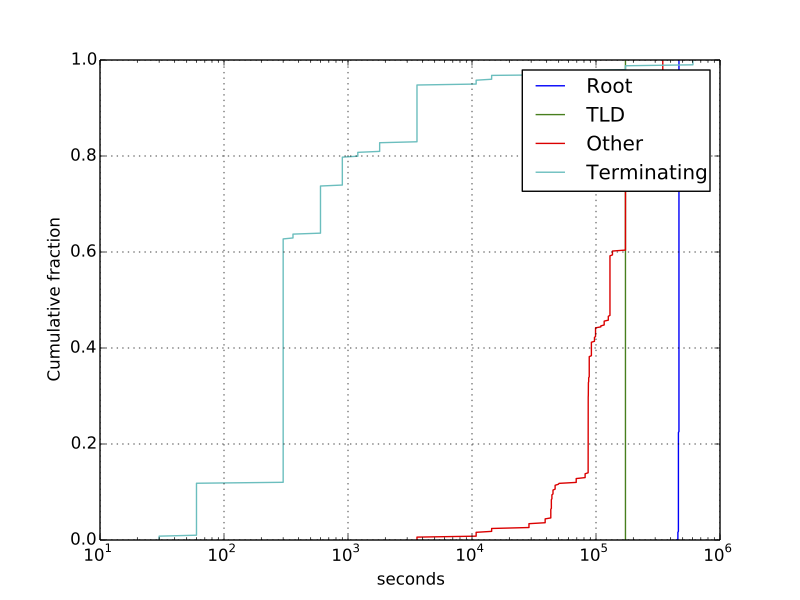
\includegraphics[scale=0.5]{example_cdf_dns_ttl}
\end{center}
FIXME: NEED THE RIGHT PLOT

\end{itemize}

\item Questions on experiment b:

\begin{itemize}

\item What are the median RTT and maximum RTT for each website? What loss rate do you observe?

\begin{center}
\begin{tabular}{ || c | c | c | c || }
\hline
Website & Median & Maximum & Loss Rate \\
\hline \hline
google.com & 2.75 & 53.0 & 0.0\% \\
\hline
todayhumor.co.kr & 79.1 & 117.0 & 0.0\% \\
\hline
zanvarsity.ac.tz & 282.0 & 452.0 & 0.0\% \\
\hline
taobao.com & 266.0 & 272.0 & 71.0\% \\
\hline
\end{tabular}
\end{center}
\newpage
\item Using the plot functions to and \texttt{rtt\_b\_raw.json}, please plot a CDF of the RTT for each website. You can plot the four CDFs on the same graph. Be sure to include a legend so we know which CDF corresponds to which of the four websites.

\begin{center}
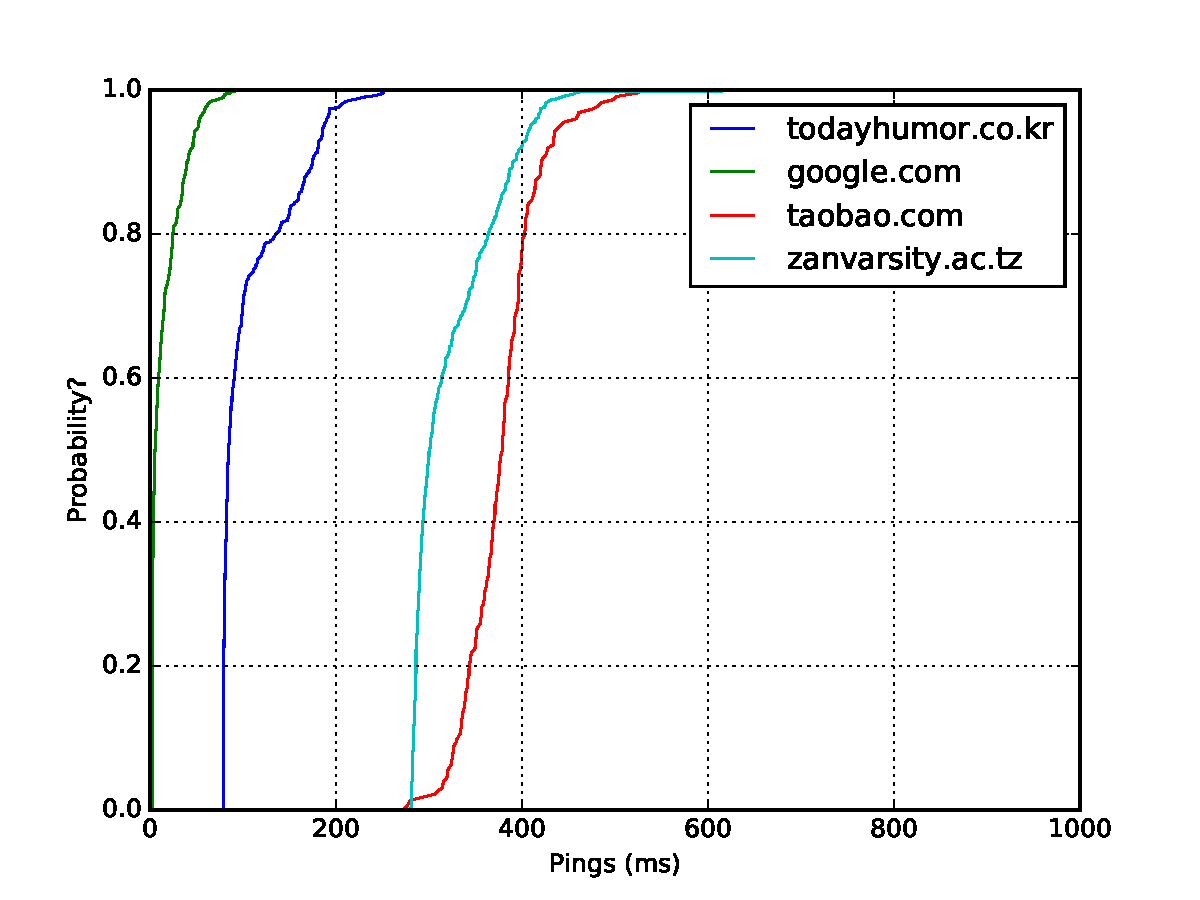
\includegraphics[scale=0.5]{rtt_b.pdf}
\end{center}
FIXME: NEED THE RIGHT PLOT

\end{itemize}

\item In this question, you will analyze the ping times to two websites and compare the results to the expected speed-of-light times. The websites are google.com (located in Mountain View, CA, USA) and zanvarsity.ac.tz (located in Zanzibar, Tanzania). You can use your ping data from experiment b. The distance from Berkeley to Mountain view is 35.23 miles, and the distance from Berkeley to Zanzibar is 9,953.50 miles.

\begin{itemize}

\item Compare the median ping time to the speed of light time. s the multiplier for each server (calculate as [ping time / speed of light time])?

\begin{center}
\begin{tabular}{ || c | c || }
\hline
Website & Ping Time / Speed of Light Time \\
\hline \hline
google.com & 14.55 \\
\hline
zanvarsity.ac.tz & 5.277 \\
\hline
\end{tabular}
\end{center}

\item Using one sentence each, list two reasons why the ping time is not equal to the speed of light time. Plausible but unlikely answers (e.a bear chewed through the wire, causing a long delay) will not receive full credit.

One reason why the ping time is not equal to the speed of light time is because switches and routers slow down transfer speeds. Another reason why the ping time is not equal to the speed of light time is because the medium the signal travels through slows it down because it isn't a vacuum.

\item \emph{[Optional]} Repeat \#3 for any website you might be curious about. How much route inflation do you observe? 

\end{itemize}
\end{enumerate}

\newpage
\subsection*{Routing}

\begin{enumerate}

\item Answer the following questions using the results obtained from experiment a

\begin{itemize}

\item Which ASes are Berkeley directly connected to?

FIXME: ANSWER HERE

\item Which traceroute traverses the most number of ASes? How about the least number of ASes?

FIXME: ANSWER HERE

\item Which websites' routes are load-balanced?

FIXME: ANSWER HERE

\item Are the observed routes stable over multiple runs? For each website, how many unique routes did you observe?

FIXME: ANSWER HERE

\item Using one sentence, please explain one advantage of having stable routes.

FIXME: ANSWER HERE

\item \emph{[Optional]} Make a graph of the ASes and their connectivity.

FIXME: ANSWER HERE

\end{itemize}

\item Answer the following questions using the results obtained from experiment b.

\begin{itemize}

\item How many hops do you observe in each route when you run traceroute from your computer? How many hops do you observe in the reverse direction?

FIXME: ANSWER HERE

\item Are these routes symmetric? How many are symmetric and how many are not?

FIXME: ANSWER HERE

\item What might cause asymmetric routes? List one or two reasons.

FIXME: ANSWER HERE

\end{itemize}
\end{enumerate}

\newpage
\subsection*{DNS}

\begin{enumerate}

\item What's the average root TTL in the 5 iterations of the top Alexa websites? Average TLD TTL? Average other name server TTL? Average terminating entry TTL?

FIXME: ANSWER HERE

\item Plot a CDF of your 5 iterations from the Alexa top 100 websites using your \texttt{generate\_time\_cdfs} function (this should have two lines, as described above).

FIXME: ANSWER HERE

\item Run \texttt{run\_dig} twice at least 1 hour apart. How many answers change within the first trial? How many names gave different answers at some point in the two trials (i.e., what values does {count\_different\_dns\_responses} return?)?

FIXME: ANSWER HERE

\item Run \texttt{run\_dig} using the name of a server in a different country. You can find public DNS servers in other countries here. 
Run \texttt{count\_different\_dns\_responses} with your original trace and the one from the new country. What does it return?

FIXME: ANSWER HERE

\item Take a look at a few of the names that returned different answers when you queried a different name server in the previous part. Use ping to measure the round trip time to the different IP addresses returned. What's the most likely reason that the different DNS server returned a different IP address? Answer in one sentence (you do not need to provide your ping output).

FIXME: ANSWER HERE

\item We asked you to use the \texttt{+trace} argument when running \texttt{dig}, which causes your local machine to resolve all requests iteratively starting from the root DNS server. How would the DNS resolution times have been different, and why if you hadn't used the \texttt{+trace} argument? Answer in 1 sentence.

FIXME: ANSWER HERE

\end{enumerate}

\end{document}